\documentclass[9pt]{beamer}


\usepackage{introLatex}
\usepackage{shortcutLatex}
\usepackage{layout}

% Dossier où se trouvent les images
\graphicspath{{imagesdiapo/}}


\newcommand{\widesim}[2][1.5]{
  \mathrel{\underset{#2}{\scalebox{#1}[1]{$\sim$}}}
  }


\begin{document}

	\begin{frame}[t]
	\titlepage
	\end{frame}


	\begin{frame}
	\vspace*{22pt}
	\tableofcontents
	\end{frame}





\footHeadLine{}

\section{Introduction du problème}

\subsection{Physique statistique et modèle d'Ising}

\setlength{\columnseprule}{0.4pt}
\begin{frame}
		\justifying
		\vspace*{22pt}

\textbf{A. Modèle d'Ising}



\begin{multicols}{2}

		$\bullet$ Modèle d'Ising 2D carré :
		\begin{itemize}
			\item Réseau carré de pas $a$.
			\item $N_s$ spins à une composantes.
		\end{itemize}
	
		
\begin{figure}[H]
\begin{center}
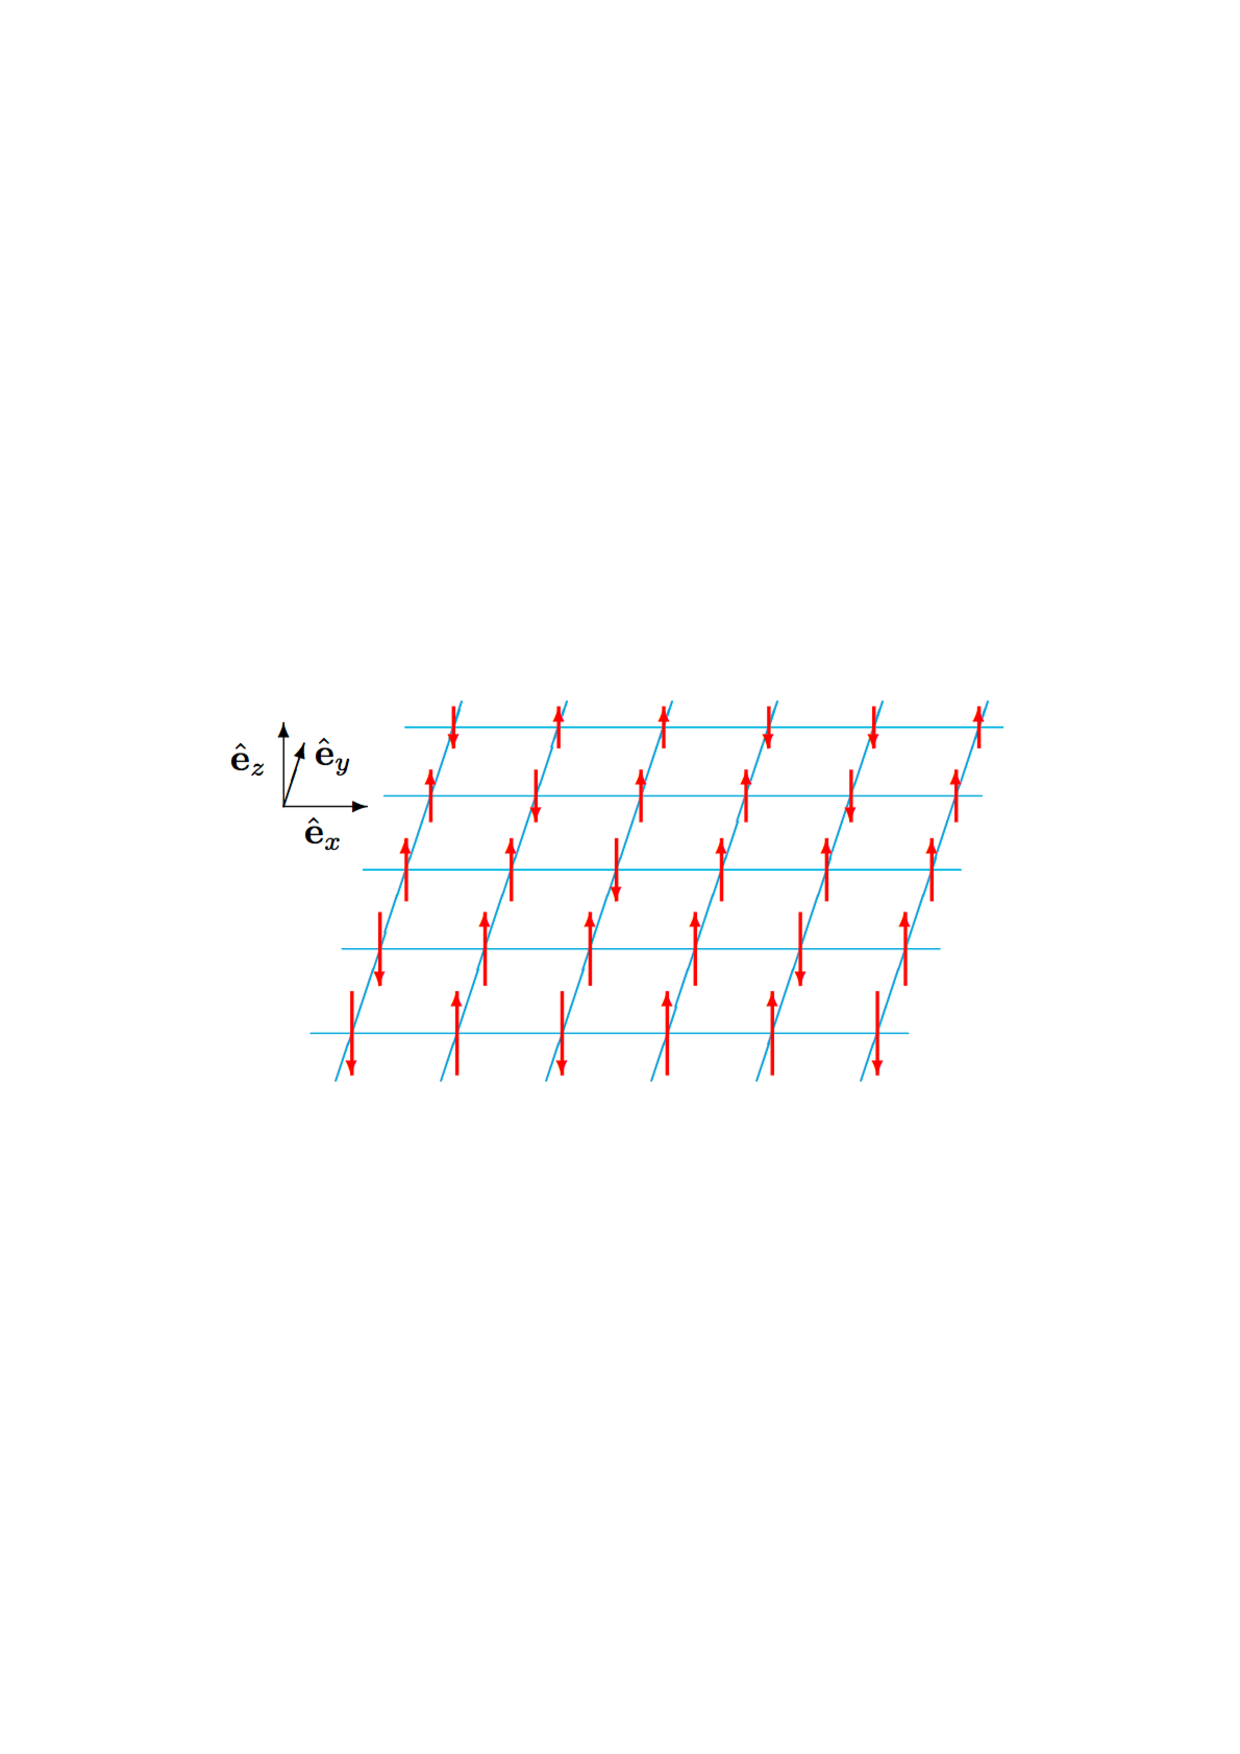
\includegraphics[scale =0.35]{Ising2D.pdf}
\caption{Modèle d'Ising.}
	\label{fig:schemaIsing}
	\end{center}
\end{figure}

$\bullet$ Spin et configuration :
\begin{equation*}
 S_\rv \in \{-1,1\}, \quad \Mr = \{S_\rv\}_\rv
\end{equation*}

$\bullet$ Energie d'une configuration $\Mr$ :
\begin{equation*}
 \Hc(\Mr) = \sum_{\left< \rv, \rv' \right>} S_\rv S_{\rv'} - \sum_\rv b_\rv S_\rv	
\end{equation*}

$\bullet$ Probabilité d'une configuration :
\begin{equation*}
p(\Mr) = \sum_\Mr \frac{1}{\Zc} \exp(-\Hc(\Mr)/(k_BT))
\end{equation*}
$\bullet$ Fonction de partition :
\begin{equation*}
\Zc = \sum_\Mr  \exp(-\Hc(\Mr)/(k_BT))
\end{equation*}

	\end{multicols}
\end{frame}

\begin{frame}
		\justifying
		\vspace*{22pt}
	$\bullet$	Définition de l'aimantation :  
		\begin{equation*}
			m = \sum_{\Mr = \{S_\rv\}_\rv } p(\Mr) \( \frac{1}{N_s} \sum_\rv S_\rv\)  = \frac{1}{N_s\beta}\partial_\beta \ln\(\Zc \) 
		\end{equation*}
		
	\onslide<2->{	
		\vspace*{11pt}
		$\bullet$ Evolution de l'aimantation $m$ avec la température $T$ :
		
\begin{multicols}{2}


	\begin{figure}[H]
\begin{center}
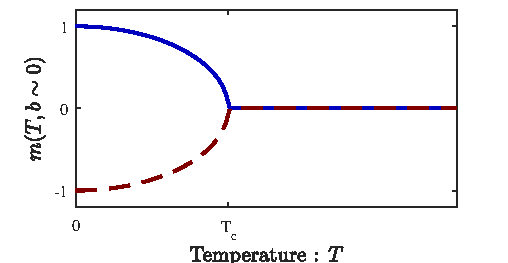
\includegraphics[width =0.95\columnwidth]{aimantation.pdf}
\caption{Aimantation $m$ vs $T$}
	\label{fig:schemaIsing}
	\end{center}
\end{figure}
	
	\vspace*{-11pt}
	Invariance par échange de $\ev_z$ en $-\ev_z$ :\\
	A $(b_\rv = 0, T=0)$  : $m=0$.\\
	\vspace*{11pt}
	
	Mais problème : 
	\begin{equation*}
		\lim_{b \to 0} \(\lim_{N_s \to \infty} m \) = 0 \neq \lim_{N_s \to \infty} \( \lim_{b \to 0} m \)
	\end{equation*}
	\end{multicols}
	}
	\vspace*{5pt}
	\onslide<3->{
	\begin{center}
$\Rightarrow$ {\Large Brisure de symétrie \& Transition de phase }
\end{center}
		}
\end{frame}
    



\subsection{Transition de phase}

	\begin{frame}
		\justifying
		\vspace*{22pt}


\onslide<1->{$\bullet$ Température critique : $T_c$} \\
\vspace*{11pt}
\onslide<2->{$\bullet$ Transitions de phase du second ordre : \\


$\quad \diamond$ Fonction de corrélation à deux points :
\begin{equation*}
\begin{split}
	G^{(2)}(|\rv_1 - \rv_2|) & \equiv \left< S_{\rv_1} S_{\rv_2} \right>   \equiv \sum_{\Mr}  p\(\Mr\) S_{\rv_1} S_{\rv_2} \, 
	\end{split}
\end{equation*}
\begin{equation*}
	\text{Pour } T = T_c, \quad	 G^{(2)}(r) \widesim{r \to \infty} |r|^{2-d-\eta}, 
\end{equation*}
$\quad \diamond$ Longueur de corrélation : 

\begin{equation*}
	\xi \widesim{T \to T_c} |T-T_c|^{-\nu} %\quad \text{et à } T = T_c, \quad	 G^{(2)}(r) \widesim{r \to \infty} |r|^{2-d-\eta}, 
\end{equation*}
}

\onslide<3->{
	\begin{center}
$\Rightarrow$ {\Large Exposants critiques : $\eta$ et $\nu$ } } \\
\end{center}

\onslide<4->{$\bullet$ {Universalité des exposants critiques }}

	\end{frame}


\setlength{\columnseprule}{0pt}
\subsection{Le groupe de renormalisation (RG)}



	\begin{frame}
		\justifying
		\vspace*{22pt}

$\bullet$ Fonction de partition exprimée avec des champs :
\begin{equation*}
	\Zc = \int \Dc \varphiv \exp\(-\Hc[\varphiv]/(k_BT)\)
\end{equation*}


\begin{multicols}{2}

$\bullet$ Transformée de Fourier :
\vspace*{-11pt}
\begin{equation*}
\begin{split}
\hat{\varphiv}_\pv = \frac{1}{\sqrt{|\Omega|}}\int_\Omega \varphiv(\rv) \, e^{-i \pv . \rv} \dd \, \rv, \\
\varphiv(\rv) = \frac{1}{\sqrt{|\Omega|}}\sum_\pv \hat{\varphiv}_\pv \, e^{i \pv  .\rv}
\end{split} 	
\end{equation*}
$ \bullet $ $\|\pv \|_2 \in [0, \Lambda]$
\vspace*{22pt}
\begin{figure}
\begin{center}
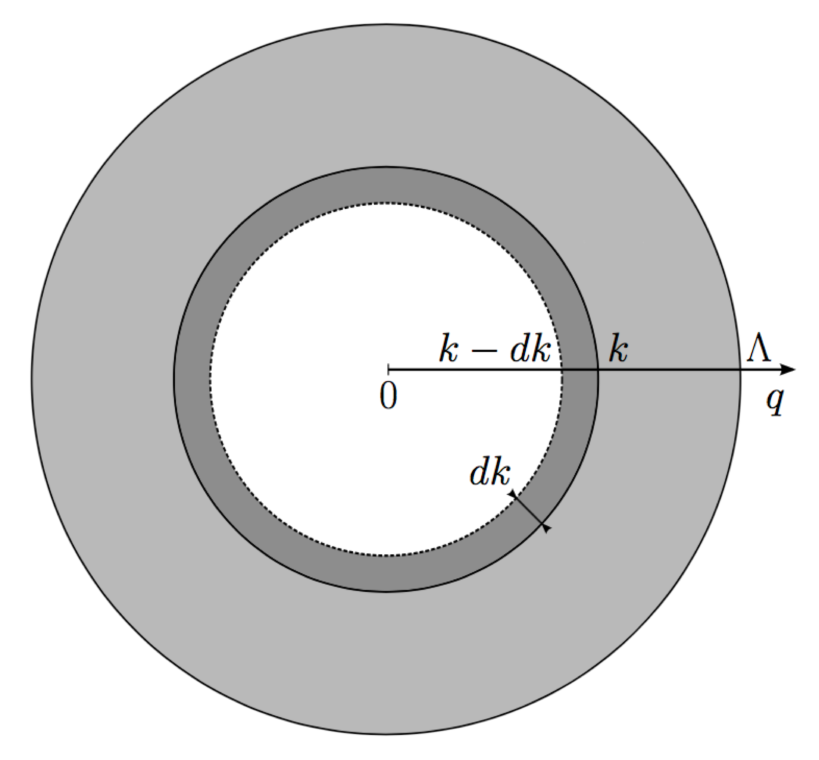
\includegraphics[scale = 0.3]{SchemaRG.pdf}
\caption{Principe du RG \\ {\footnotesize \textit{Thèse de Frédéric Léonard}}}
	\label{fig:SchemaRG}
	\end{center}
\end{figure}

\end{multicols}

	$\bullet$ En pratique :  $\Zc_k \underset{\text{NPRG}}{\longrightarrow} \Gamma_k   \underset{\text{BMW}}{\longrightarrow} \Gamma^{(2)}_k$
	\end{frame}
	

	
	
	\subsection{Les équations BMW}

	\begin{frame}
		\justifying
		\vspace*{22pt}
L'équation de flot BMW : 
\begin{equation*}
\begin{split}
	\partial_t \Gamma_{k}^{(2)}(\pv, \phi) & = J_3(\pv, \phi) {\( \partial_\phi \Gamma_{k}^{(2)}(\pv, \phi) \)}^2  - \frac{1}{2}  I_2(\phi) \, \partial_\phi^{2} \Gamma_{k}^{(2)}(\pv, \phi)
\end{split}
\label{eq:flotBMW}
\end{equation*}
Avec les notations,
\begin{equation*}
\begin{split}
	J_n(\pv,\phi) & = \int_\qv \partial_t \Rc_k(\qv) \,G_k(\pv+\qv, \phi) \,G_k^{n-1}(\qv, \phi) \, ,  \\
	I_n(\pv,\phi) & = \int_\qv \partial_t \Rc_k(\qv) \,G_k^{n}(\qv, \phi) \, .
\end{split}
\label{eq:JI}
\end{equation*}
Définition du propagateur :
\begin{equation*}
G_k(\qv, \phi) = \frac{1}{\Gamma_k^{(2)}(\qv,\phiv)+ \Rc_k(\qv)}	
\end{equation*}
Condition initiale en $k = \Lambda$ connue
	\end{frame}
    
    
    \subsection{Objectif}
    \begin{frame}
		\justifying
		\vspace*{22pt}
    
    \onslide<1->{$\Rightarrow$ {\Large Calcul des exposants critiques : $\eta$ et $\nu$ } }\\
    \onslide<2->{$\Rightarrow$ {\Large Calcul de la température critique : $T_c$ }} \\
    
    \vspace*{11pt}
    
    \onslide<3->{
    $\bullet$ Première étude :\\
    \begin{itemize}
    \item Réecriture en C++ d'un code permettant de calculer $\eta$ et $\nu$
    \item Recherche des problèmes et tentatives de résolution
    \end{itemize}
    }
    
    \vspace*{11pt}
    
    \onslide<4->{
    $\bullet$ Deuxième étude :\\
    \begin{itemize}
    \item Ecriture d'un nouveau code pour calculer $T_c$ : faisable  mais difficile
    \item Comparaison à la valeur théorique : benchmarking de la méthode
    \end{itemize}
    }
    
    \end{frame}

    
    

    
    \section{Le problème continu}
    \subsection{Hamiltonien du modèle continu $\varphiv^4$}
    
        \sommaire{}
    
    
      \begin{frame}
		\justifying
		\vspace*{22pt}
    
    \begin{equation}
		H[\varphiv] = \int_\rv \, \left\{ \frac{1}{2}(\nabla \varphiv)^2 + \frac{1}{2}r_0 \varphiv^2 + \frac{u_0}{4!}{\({\varphiv}^{2}\)}^{2} \right\}
		\label{eq:hamiltCont}
\end{equation}
    	\end{frame}
    
    
    \subsection{Système d'équations à résoudre}
    
    
    \begin{frame}
		\justifying
		\vspace*{22pt}

{\itshape Trouver $(\tY_k,\tW_k)$ tel que pour tout $k \in ]0 ,\Lambda]$,  $\trho \in [0, +\infty[$ et $\tp \in [0, +\infty[$,}
\begin{align*}
	\partial_t  \tY_k(\tp, \trho) & = 
	\begin{aligned}[t]
			& \eta_k(1+\tY_k(\tp, \trho)) + \tp \, \partial_{\tp} \tY_k(\tp, \trho)  -(2-d-\eta_k)\trho \,\partial_{\trho} \tY_k(\tp, \trho)  \quad  \\
			& + 2\trho \tp^{-2} \left[ {\( \tp^2 \partial_{\trho} \tY_k(\tp, \trho) + \tilde{u}_k(\trho)\)}^2\, \tJ_3(\tp, \trho) \right]  - 2\trho \tp^{-2} \left[ \tilde{u}_k^2(\trho)  \tI_3(\trho) \right] \\
			&  - \tI_2(\trho) \(  \partial_{\trho} \tY_k(\tp, \trho) / 2 + \trho \,  \partial_{\trho}^2 \tY_k(\tp, \trho) \)
	\end{aligned}
	\label{eqn}\\
	\partial_t  \tW_k &  = 
	\begin{aligned}[t]
		& (\eta_k-2) \tW_k(\trho) + (d-2+\eta_k) \trho \,\partial_{\trho}\tW_k(\trho) + \frac{1}{2} \partial_{\trho} \tI_1(\trho) \, ,
	\end{aligned}
\end{align*}
\textit{avec la définition}
\begin{equation*}
\begin{split}
\eta_k = \frac{1}{2}  \tI_2(\trho = 0)\partial_\rho\tY_k(\tp = 0, \trho = 0) \,, 
\end{split}
\end{equation*}
\textit{et les conditions initiales,}
\begin{equation*}
	\tY_\Lambda(\tp, \trho) = 0 \quad  \text{et} \quad \tW_\Lambda(\trho) = \tilde{r}_0 + \tilde{u}_0\trho
\end{equation*}

	\end{frame}
	

	\subsection{Méthodes numériques}
	
	
     \begin{frame}
		\justifying
		\vspace*{22pt}
    
    
   	\onslide<1->{$\bullet$ Discrétisation en temps : Schéma d'Euler explicite} \\
   	\onslide<2->{$\bullet$ Discrétisation en champ : Grille fixe. Dérivée avec schémas à 5 points}\\
   	\onslide<3->{$\bullet$ Discrétisation en moments : Méthode pseudo-spectrale
   	\begin{itemize}
   		\item Interpolation de Tchebytechev	
   		\item Intégration de Gauss-Legendre
   	\end{itemize}
 } 	
   	\vspace*{11pt}
   
   \onslide<4->{	
   	$\bullet$ A propox de l'intégration
   	\begin{equation*}
K = \int_{\R^d} f(\tqv^2)g((\tpv+\tqv)^2) \, \dd \, \tqv \, ,
\end{equation*}
\begin{equation*}
K = S_{d-1} \int_0^{+\infty} \dd\tq_2 \, \tq_2^{d-2} \int_{-\infty}^{+\infty} \dd\tq_1 \, f(\tq_1^2 + \tq_2^2) g(\tp^2 + \tq_1^2 + \tq_2^2 + 2\tp\tq_1)
\end{equation*}

}
	\end{frame}
	
	
	
	\subsection{Résultats}
	
	   \begin{frame}
	\justifying
	\vspace*{22pt}

	
	
	\end{frame}
	
	
	
	\section{Le problème du modèle d'Ising 2D}
    	
    	\subsection{Mise en équations}
    	
    	\sommaire{}
   	
	   \begin{frame}
	\justifying
	\vspace*{22pt}

	$\bullet$ Réecriture de la fonction de partition :
	
	\begin{equation}
  \Zc  \propto \int_\R \prod_{\rv} \, \dd \varphi_\rv \, \exp\(-\Hc_\mu[\varphi] \) \, ,
\end{equation}
avec l'hamiltonien $\Hc_\mu$ définit par 
\begin{equation}
  \Hc_\mu[\varphi] = \frac{1}{2} \int_\qv \varphi(\qv) \frac{1}{\lambda_\mu(\qv)} \varphi(-\qv) - \sum\limits_\rv \ln\(\cosh(\varphi_\rv)\) \, ,
\end{equation}
	
	\end{frame}
	
	\begin{frame}
	\justifying
	\vspace*{22pt}

	$\bullet$  :
	
	\end{frame}
	
	
	\subsection{}
	
	\begin{frame}
	\justifying
	\vspace*{22pt}

	$\bullet$ Réecriture de la fonction de partition :
	
	\end{frame}
	

\end{document}